
%(BEGIN_QUESTION)
% Copyright 2013, Tony R. Kuphaldt, released under the Creative Commons Attribution License (v 1.0)
% This means you may do almost anything with this work of mine, so long as you give me proper credit

The following Allen-Bradley PLC program controls the operation of a machine using a {\it sequencer} (SQO) instruction.  Unfortunately, the system seems to be having a problem as the machine is ``stuck'' at one step in its sequence.  Your first step is to connect a laptop PC to the PLC and monitor the ``online'' status of its program.  What you see on the laptop screen is this, unchanging:

$$\includegraphics[width=15.5cm]{i03359x01.eps}$$

Based on this information, what do you suppose is the most likely fault?  What would be your next diagnostic step?

\underbar{file i03359}
%(END_QUESTION)





%(BEGIN_ANSWER)

The give-away here is that timer {\tt T4:0} is stuck at its present accumulator value of 3 despite being enabled to time with all the sufficient conditions present.  This means the PLC program execution has been halted for some reason.  This may be the result of the processor being placed in ``Stop'' mode (instead of ``Run'') or perhaps a ``Fault'' condition within the processor caused by something such as a math calculation error (e.g. divide by zero).
 
\vskip 10pt

A good ``next step'' to take would be to look at the laptop's indication of processor run status.  Is there a red ``Fault'' condition shown?  Has the processor been placed into ``Stop'' mode?  Perhaps is this section of code found in a subroutine that is not being called for some reason by the main program?

%(END_ANSWER)





%(BEGIN_NOTES)


%INDEX% PLC, troubleshooting: sequencing control system

%(END_NOTES)


